%\section{Object flow}
\subsection{Flow estimation}
\label{sec:core}

The object flow consist on computing the motion field for an object of interest through an image
sequence. The most usual approach to solve a problem like this is to implement some of the available
optical flow techniques through the complete sequence and perform the flow integration. 
However, this process results in high levels of motion drift \cite{c18}\cite{c19} and usually the motion of the interest
object is affected by a global regularization. In some extreme cases, the interest object motion
may be totally blurred and other techniques have to be incorporated. Moreover, the diversity
of natural video sequences makes difficult the choice of one technique over another, even when specialized
databases are at hand \cite{c17}, because currently no single method can achieve a strong 
performance in every of the available datasets. Most of these methods consist in the minimization 
of an energy function with two terms (As was previously mentioned in the Sec. \ref{sec:suppix}). The data
term is mostly shared between different approaches, but the prior or spatial term is different, and basically states 
under what conditions the optical flow smoothness should be maintained or not. In a global approach, however,
this is a difficult concept to define. Most of these smoothness terms rely in appearance differences or gradients.
All these meaning that, unavoidably, some methods may be more reliable for some cases but weaker for others. 
It can be argued that this behaviour may be caused because most of the techniques do not count with a way to identify 
firmly where exactly this smoothness prior can be applied. 

\ifcsdef{r@accv_format}{
   \begin{figure}[thpb]
      \centering
      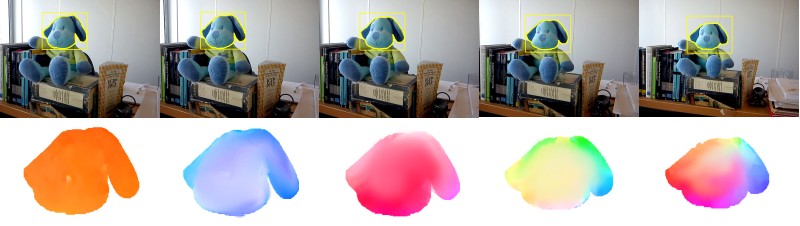
\includegraphics[width=1.0\textwidth]{../images/objectflow.png}
      \caption{Object flow with the color code of \cite{c17} (bottom) for frames in the Puppy sequence (up). }
      \label{of}
   \end{figure}
}{
   \begin{figure}[thpb]
      \centering
      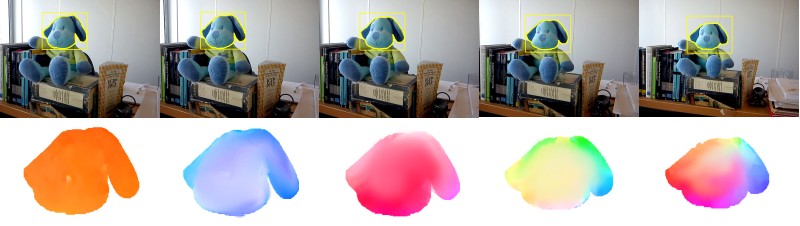
\includegraphics[width=0.5\textwidth]{../images/objectflow.png}
      \caption{Object flow with the color code of \cite{c17} (bottom) for frames in the Puppy sequence (up). }
      \label{of}
   \end{figure}
}
The main idea behind the object flow is that given the availability of several robust tracking techniques, and the proposed
segmentation method for video, the optical flow computation can be refined by computing it successively between pairs
of tracked windows. The basic proposal to perform this refinement consist on considering the segmentation limits  as reliable smoothness boundaries. 
This is, of course, under the assumption that the motion is indeed smooth within the object region. 
This is assumption is not far from reality in most scenes with an interest object. 
Naturally, as the object tracker is included, is expected that the object flow should be more robust to rapid motions than the
optical flow. 
Thus, the full motion is split in two, the long range motion, given by the tracker window, and the precision part, given by the targeted optical flow. The Fig. \ref{of} shows 
the object flow for a frame in the Puppy sequence. Observe the motion vectors are computed only inside the object of interest, preserving a strong smoothing prior, but 
also allowing internal variations in the flow. 

As a first approximation to the object flow, the Simple Flow technique \cite{c21} is taken as core base. This is because of its scalability 
to higher resolutions and because its specialization to the concept of object flow is only natural. This is because in the Simple Flow pipeline 
the smoothness localization can be easily specified through computation masks. More specifically, the initial computation mask is derived from 
the segmentation performed as prior step. The resulting flow is then filtered only inside the mask limits to enhance precision and fastening the 
implementation. However, direct modifications in other optical flow methods can be further studied. For instance, in graph-cut based 
minimization approaches, the regularity constraints can be precisely targeted by disconnecting foreground pixels from background ones.

\section{Experimental results}
\ifcsdef{r@accv_format}{
   \begin{figure}[th]
      \centering
      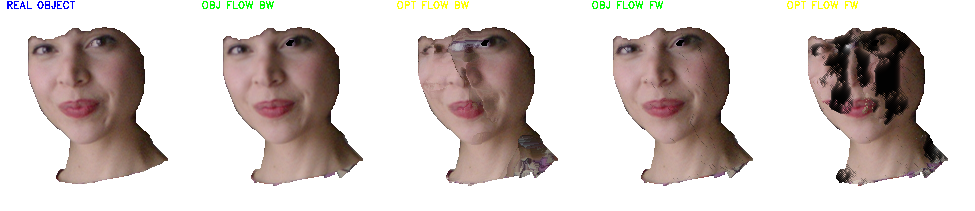
\includegraphics[width=1.00\textwidth]{../images/extrapolated.png}
      \caption{Extrapolation results from integrated flow in 4 sequences. In descending order: Amelia Retro, Boy, Walking, Puppy. From Left to Right: Annotated object, Backward object flow, Backward optical flow, Forward object flow, Backward optical flow.}
      \label{sample}
   \end{figure}
	\setlength{\belowcaptionskip}{-10pt}
}{
   \begin{figure}[th]
      \centering
      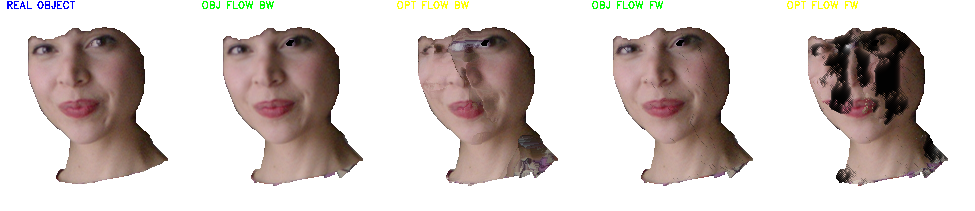
\includegraphics[width=0.5\textwidth]{../images/extrapolated.png}
      \caption{Extrapolation results from integrated flow in 4 sequences. In descending order: Amelia Retro, Boy, Walking, Puppy. From Left to Right: Annotated object, Backward object flow, Backward optical flow, Forward object flow, Backward optical flow.}
      \label{sample}
   \end{figure}
	\setlength{\belowcaptionskip}{-10pt}
}
To evaluate the performance of the object flow in comparison with optical flow techniques, we performed 
a number of experiments on several video sequences. We annotated an initial bounding box for the videos, 
and a segmentation contour of the interest object for every frame. The experiment measures the ability of the method to 
extrapolate an image from the initial frame and the integrated flow. For every pair of frames the video sequence, the PSNR between the annotated
current state of the object and the extrapolated images is computed. The Fig. \ref{sample} is a sample of the performed experiment, each column is an image generated from the given flow. 
Two types integration are evaluated, $From-the-reference$, or forward integration, and $To-the-reference$, or backward integration, as discused in \cite{c20}. So, for each row in the Fig. \ref{sample}, two columns correspond to the object flow, and two columns correspond to optical flow, with both types of integration.

The Fig. \ref{of_res} shows PSNR graphics for 4 different sequences. For every pair of frames an image is extrapolated, and the PSNR with the ground-truth object is computed.
The results are shown with both, Euler integration (Labelled as $forward$ in the figs.) of the used flow, 
and using the integration method described in \cite{c20}, labeled as $backward$ in the figures. The results show that the object flow methods are generally more precise than its optical flow 
counterparts. Moreover, the object flow method with backward integration usually performs much better than any other combination of techniques. For this experiment, the object flow is compared with the simple-flow optical-flow method.

\ifcsdef{r@accv_format}{
   \begin{figure}[hb]
      \centering
      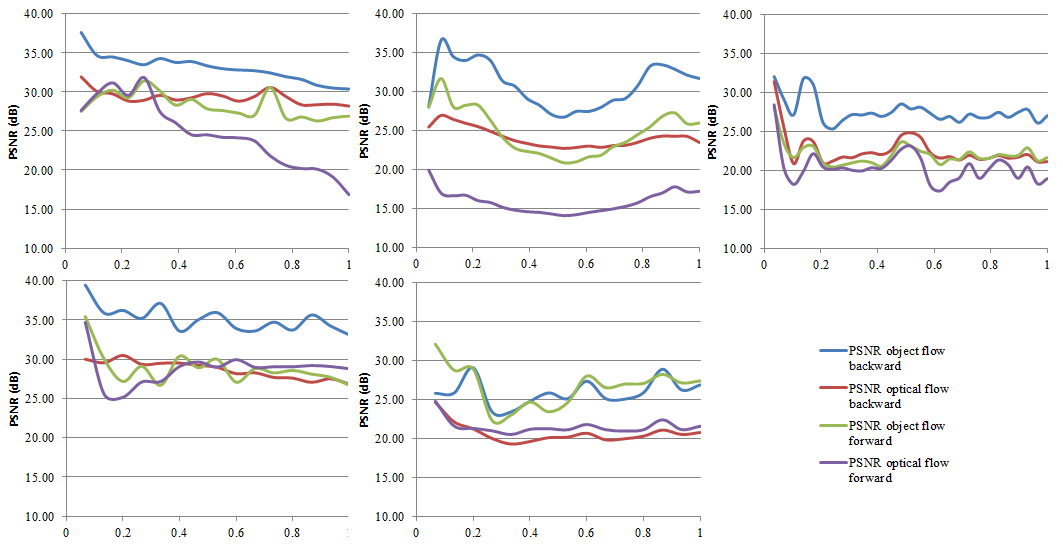
\includegraphics[width=1.0\textwidth]{../images/psnr.png}
      \caption{PSNR graphs for extrapolated images using Object flow and the Simple Optical Flow for 4 sequences. In descendent order: Puppy Seq.; Amelie Retro Seq.; Boy Seq.; Walking Seq.}
      \label{of_res}
   \end{figure}
	\setlength{\belowcaptionskip}{-10pt}
}{
   \begin{figure}[hb]
      \centering
      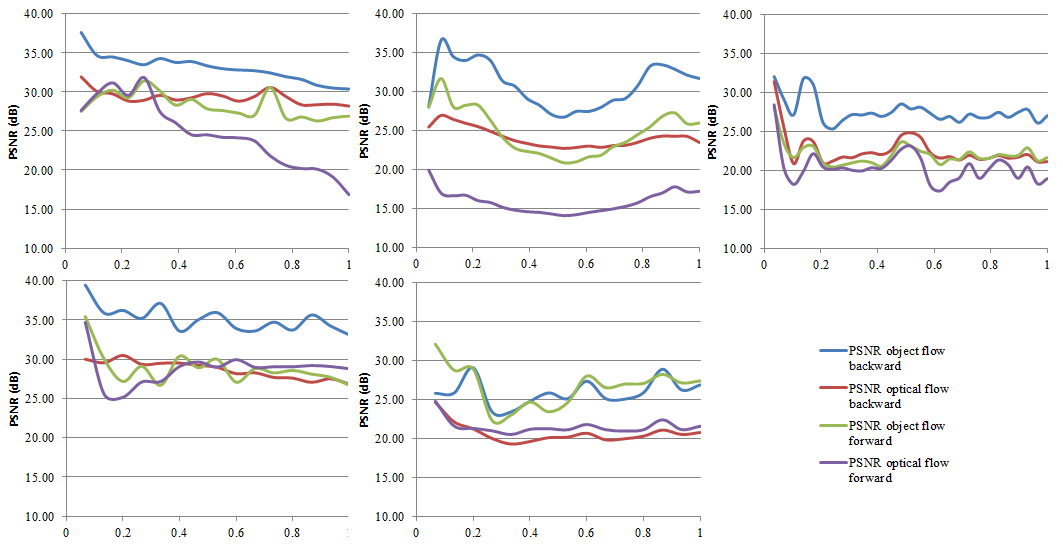
\includegraphics[width=0.5\textwidth]{../images/psnr.png}
      \caption{PSNR graphs for extrapolated images using Object flow and the Simple Optical Flow for 4 sequences. In descendent order: Puppy Seq.; Amelie Retro Seq.; Boy Seq.; Walking Seq.}
      \label{of_res}
   \end{figure}
	\setlength{\belowcaptionskip}{-10pt}
}

The Fig. \ref{compare2} presents a visual comparison between the object flow and several optical flow techniques in the Amelia sequence for object extrapolation, and the involved frames (the first and last used frames in the sequence). The Fig. \ref{of_res2} shows the PSNR results for every extrapolated frame in the full sequence, the object flow performs better 
than all the studied optical flow techniques.

\ifcsdef{r@accv_format}{
   \begin{figure}[t]
      \centering
      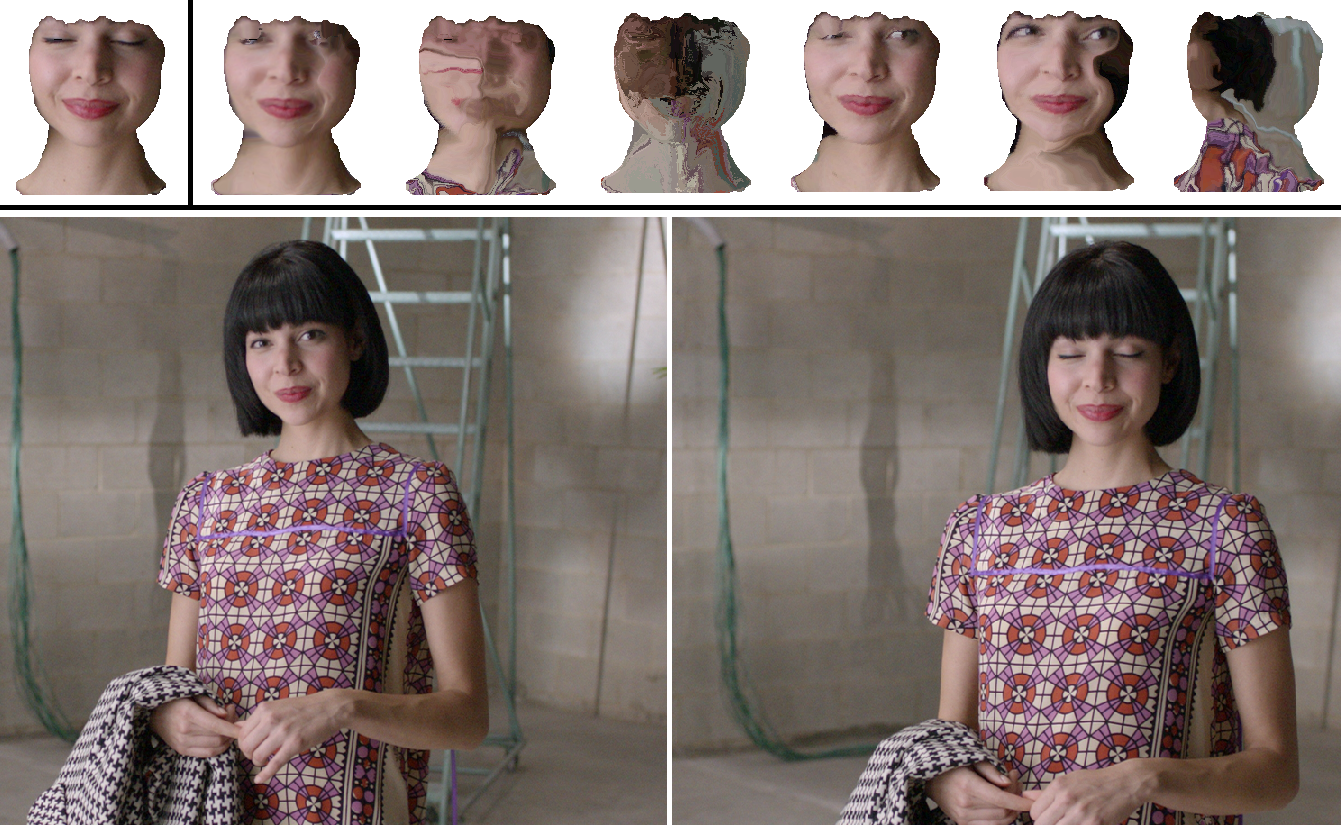
\includegraphics[width=1.0\textwidth]{../images/compare2.png}
      \caption{Top: Comparison between extrapolated objects using several methods: Groundtruth object, Object flow, TVL1, Block Matching, Brox, Farneback and Simple Flow. 
		Bottom: First and current frame. The extrapolation is performed using backward accumulation of the flow.}
      \label{compare2}
   \end{figure}
	\setlength{\belowcaptionskip}{-10pt}
}{
   \begin{figure}[t]
      \centering
      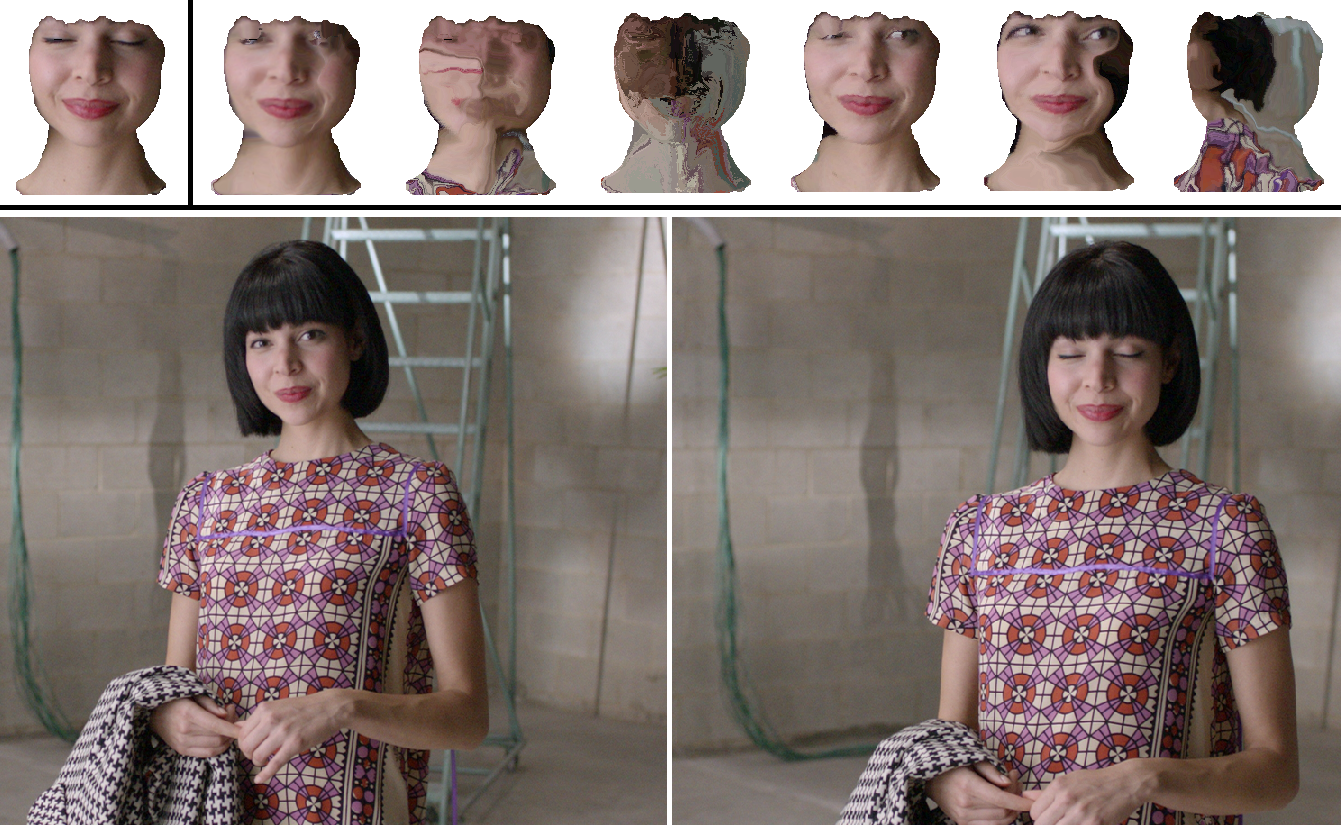
\includegraphics[width=0.5\textwidth]{../images/compare2.png}
      \caption{Top: Comparison between extrapolated objects using several methods: Groundtruth object, Object flow, TVL1, Block Matching, Brox, Farneback and Simple Flow. 
		Bottom: First and current frame. The extrapolation is performed using backward accumulation of the flow.}
      \label{compare2}
   \end{figure}
	\setlength{\belowcaptionskip}{-10pt}
}

Observe that the object details are lost in comparison with the ground-truth object image (Fig. \ref{compare2}). For example, the closed eyes detail is missing in the most of the optical 
flow methods. Furthermore, several of the methods lost any significance, and the output barely holds any resemblance with the original image.

\ifcsdef{r@accv_format}{
   \begin{figure}[th]
      \centering
      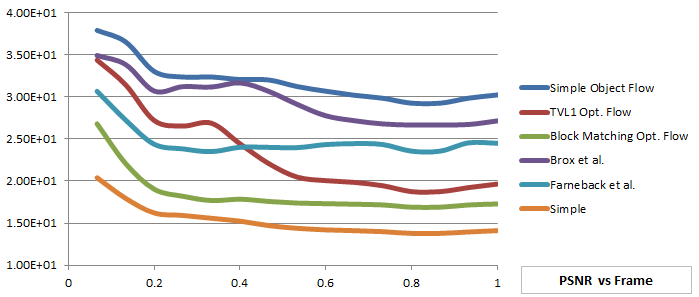
\includegraphics[width=1.0\textwidth]{../images/psnr2.png}
      \caption{PSNR graphs for extrapolated images using Object flow and the different Optical Flow techniques for the Amelia sequence. }
      \label{of_res2}
   \end{figure}
	\setlength{\belowcaptionskip}{-10pt}
}{
   \begin{figure}[th]
      \centering
      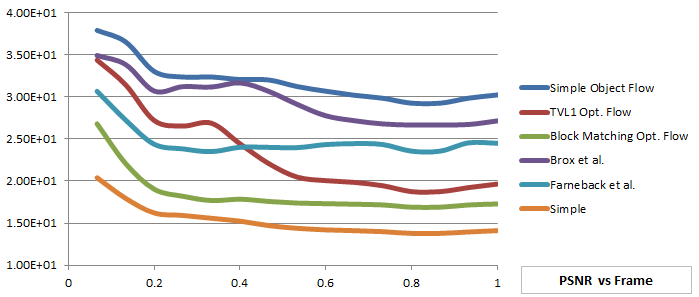
\includegraphics[width=0.5\textwidth]{../images/psnr2.png}
      \caption{PSNR graphs for extrapolated images using Object flow and the different Optical Flow techniques for the Amelia sequence. }
      \label{of_res2}
   \end{figure}
	\setlength{\belowcaptionskip}{-10pt}
}